\clearpage

\subsection{Tenho Dito}

``Tenho Dito'' corresponde ao produto deste trabalho visível pelo usuário final. Trata-se de uma aplicação \textit{web}, desenvolvida utilizando a linguagem \textit{python} com o \textit{framework Django}, e tem como objetivo ser uma forma mais lúdica e amigável de visualização de alguns dados disponíveis nos \textit{webservices} de dados abertos da Câmara dos Deputados. Utiliza métodos de processamento de linguagem natural e aprendizado de máquina para extrair o perfil temático dos parlamentares, analisando o texto de seus discursos e proposições. Além disso, também é possível traçar os temas mais discutidos (tanto em propostas quanto nos próprios discursos) pelos deputados de uma determinada região ou por partidos.

A aplicação é dividida em dois grandes módulos: \textit{nlp} e \textit{application}. O primeiro é responsável por todas as operações relacionadas ao processamento dos textos, o que inclui aprendizado de máquina. Já o segundo módulo é responsável pela parte \textit{web}. No momento de escrita desse trabalho, foi implementado apenas a principal funcionalidade do produto: a análise por estado. E estão disponíveis alguns protótipos de tela, mostrando as possíveis funcionalidades do sistema.

Conforme mencionado no item ``\textit{frameworks}'', em \ref{ferramentas}, a análise dos textos será realizada com o apoio das ferramentas:

\begin{itemize}
    \item \textbf{Plagiarism:} biblioteca em estado \textit{alpha} desenvolvida pelo professor orientador do autor desse trabalho, Fábio Macêdo Mendes, e possui uma série de funcionalidades utilizadas no pré-processamento dos textos, como extração de \textit{tokens}, \textit{stemização}, remoção de \textit{stop words}, geração de \textit{n-gramas} e geração de \textit{bag-of-words} (com os diferentes tipos de representação dos termos, descrito na seção \ref{sec:representação_dos_termos} desse trabalho). Apesar do foco ser a detecção de plágio em textos e códigos, as funcionalidades implementadas podem ser utilizadas em tarefas genéricas de PLN.
    \item \textbf{Textblob:} biblioteca \textit{python} para processamento de dados textuais. Ela fornece uma interface simples para realizar tarefas comuns de processamento de linguagem natural, como análise de sentimento e classificação, por exemplo. Utiliza a biblioteca \textit{NLTK}\footnote{http://www.nltk.org} para realizar essas tarefas.
\end{itemize}

Com o objetivo de deixar registrado as experiências obtidas na primeira parte desse trabalho, dividimos essa seção em duas partes.

\subsubsection{Primeira Parte do Trabalho}

Na primeira parte desse trabalho, a classificação dos discursos e proposições era dividida em duas etapas. A primeira etapa consistia em, inicialmente, dividir o texto em parágrafos, para que a análise fosse realizada com uma quantidade menor de texto, e em seguida os parágrafos seriam classificados entre ``conteúdo útil'' ou ``conteúdo não-útil''. Por exemplo, o trecho \textit{``Muito obrigado, nobre Deputado. Pelo PSOL de São Paulo, o nobre Líder Ivan Valente. V. Exª tem cinco minutos na tribuna.''} não representa um conteúdo significativo, da mesma forma que `\textit{`O SR. ALCEU MOREIRA - Sr. Presidente, primeiro a medida provisória, logicamente.''} também não agregaria nenhum valor à análise. Trechos como esses deveriam ser classificados como ``conteúdo não-útil'' e descartados da análise temática. A segunda etapa do processamento era a classificação temática dos parágrafos classificados como ``conteúdo útil'', na etapa anterior.

Para ambas etapas o procedimento adotado era o mesmo, com algumas alterações nos classificadores. Primeiro, um classificador \textit{NaiveBayesClassifier}, implementado pela biblioteca \textit{textblob}, era instanciado, utilizando dois conjuntos de palavras iniciais, um para definir ``conteúdo não-útil'' e outro para ``conteúdo''. Os conjuntos de palavras podem ser encontrados no apêndice \ref{conjunto-palavras}.

Em seguida, todos os parágrafos eram classificados e, dentre os que foram classificados com uma probabilidade maior que 80\%, os 100 melhores colocados eram utilizados para realizar o treinamento inicial do classificador. A partir disso, era realizado um treinamento supervisionado, onde a aplicação sugeria uma classe mais provável e um especialista humano dizia se o trecho correspondia à classe sugerida, caso não fosse ele deveria fornecer a classe correta. Ao finalizar o treinamento supervisionado, todos os parágrafos eram classificados novamente, agora com o classificador melhor treinado.

Vale observar que as classificações útil/não-útil sugeridas após a primeira fase normalmente correspondiam às corretas, ainda que isto não tenha sido medido explicitamente.

Com o resultado a primeira classificação, obtinha-se um conjunto de parágrafos classificados como ``conteúdo'', que seriam usados na classificação temática. De forma semelhante à primeira classificação, um classificador \textit{NaiveBayesClassifier} era instanciado, agora com um conjunto de palavras específico para cada tema. Os temas e seus respectivos conjuntos de palavras também se encontram no apêndice \ref{conjunto-palavras}.

Todos os parágrafos eram classificados novamente e era gerado um conjunto com os melhores classificados, que era usado para realizar o treinamento inicial do classificador. Após esta etapa, acontecia o treinamento supervisionado, onde um especialista dizia se a classificação sugerida fazia sentido e indicava a classe correta quando não fosse.

Também era possível realizar um treinamento não supervisionado para ambos os classificadores, de forma que as sugestões de classificação eram utilizadas para o treinamento sem a análise de um especialista.

A cada iteração da fase de treinamento todas as probabilidades dos textos adicionados ao classificador são recalculadas, o que implica no aumento significativo do tempo de processamento. Por isso, foi utilizada uma ferramenta de \textit{cache}, possibilitando o armazenamento dos classificadores depois de cada atualização. Toda vez que for realizado um treinamento ou uma classificação seria utilizado o último classificador armazenado em \textit{cache}, com o treinamento prévio.

Esta fase mostrou que alguns discursos são difíceis de classificar ou por terem um conteúdo fragmentado (ex.: parágrafo com apenas uma ou poucas palavras, como \textit{``-Rio de Janeiro''}) ou por conter um conteúdo que aborda mais de um tema simultaneamente (ex.: \textit{``Eu parei de jogar há quase 17 anos e há 15 anos eu criei o Instituto Esporte \& Educação - IEE, do qual sou Presidente, que trabalha com esporte e educação. E há 15 anos nós viajamos para cidades do Brasil que não têm acesso à prática motora na escola, que não têm estrutura, que não têm professores e, especialmente, que não têm a visão da educação física, do esporte, do movimento, da ação motora, da atividade motora como um fator de desenvolvimento, cuja presença é importante dentro da escola.''}).

\subsubsection{Segunda Parte do Trabalho}

Tendo em vista que o resultado das classificações utilizando o modelo descrito acima não foi satisfatório, algumas alterações foram feitas. Tais alterações serão organizadas por tópicos.

\paragraph{Dados Utilizados na Análise}

Em primeiro lugar, passamos a utilizar uma base de palavras pré-classificadas maior: o \textit{thesaurus} da Câmara dos Deputados, que estará disponível no repositório do Tenho Dito. Esse conjunto de palavras foi utilizado para treinamento do classificador, o que melhorou, mas não o suficiente, o resultado da classificação temática.

Também deixamos de utilizar o texto completo para a análise e passamos a utilizar apenas o sumário, que é basicamente um resumo do discurso/proposição estruturado de forma simples, onde cada sentença corresponde a um tópico abordado pelo deputado (geralmente). Temos, por exemplo, o sumário de um discurso proferido pelo deputado Alberto Fraga, no dia 10/07/2017: \textit{``Incompetência administrativa do Governador Rodrigo Rollemberg. Protesto contra a derrubada de construções na orla do Lago Paranoá, determinada pelo Governo de Brasília. Repúdio à ação ajuizada contra o orador, em face de críticas à administração do Distrito Federal.''}. Analisando o sumário, podemos ver que \textit{``Incompetência administrativa do Governador Rodrigo Rollemberg''} aborda um tema, \textit{``Protesto contra a derrubada de construções na orla do Lago Paranoá, determinada pelo Governo de Brasília''} aborda outro e \textit{``Repúdio à ação ajuizada contra o orador, em face de críticas à administração do Distrito Federal.''} outro. Essa característica permitiu o descarte do primeiro classificador (de ``conteúdo útil/não-útil'') e melhorar um pouco a classificação temática, já que as sentenças obtidas trazem um conteúdo relevante, são menores e abrangem menos temas.

Entre os dados de proposições disponíveis no \textit{webservice} de dados abertos da Câmara dos Deputados não encontramos algo semelhante ao sumário dos discursos, apenas a ementa da proposição, mas que na maioria das vezes contém algo muito técnico, sendo necessário o conhecimento mais profundo das leis, como por exemplo: \textit{``Revoga os artigos 165, 166 e 204 do Decreto-Lei nº 1.001, de 21 de outubro de 1969.''}. Buscando utilizar os mesmos dados, tanto para discursos quanto para proposições, optou-se pela utilização da indexação realizada pela Câmara dos Deputados, já que a mesma está presente em todos os discursos realizados no Pequeno Expediente e em todos os Projetos de Lei. Somente para exemplificar, o Projeto de Lei que possui a ementa citada anteriormente, possui a seguinte indexação: \textit{``Revogação, dispositivo legal, Decreto-Lei, Código Penal Militar, promoção, reunião, publicação, crítica, indevido, exercício, comércio, militar da ativa''}, o que permite o entendimento do que realmente a proposição aborda.

\paragraph{Modelos Utilizados}

Na primeira parte desse trabalho, tentou-se utilizar uma abordagem não-supervisionada com o \textit{k-means} e ao não obter um resultado satisfatório, optou-se pela utilização do \textit{Naive Bayes}. Este, por sua vez, define apenas uma classe para cada texto analisado, mesmo quando o texto aborda mais de um tema. Com o objetivo de identificar mais de um tema por discurso, iniciou-se o estudo do modelo \textit{LDA}.

O \textit{LDA} é, naturalmente, não-supervisionado. Entretanto, a implementação da biblioteca \textit{Gensim}\footnote{\lnk{Gensim}{https://radimrehurek.com/gensim/models/ldamodel.html\#gensim.models.ldamodel.LdaModel}} permite inserir informações a priori no algoritmo.

Para aplicar o \textit{LDA}, instanciamos um objeto da classe \textit{LdaModel} passando como parâmetros o \textit{corpus} de treinamento utilizado (\textit{thesaurus}), a quantidade de tópicos a serem encontrados e o \textit{eta}, que será utilizado pelo algoritmo para definir probabilidades a priori. O \textit{eta} é uma matriz \(K \times n\), onde \(K\) é o número de tópicos e \(n\) o número de termos. Com essa matriz, podemos definir valores específicos para determinadas palavras em relação aos tópicos, sendo que o valor padrão para cada palavra é de \(\frac{1}{K}\). Dessa forma, os termos já classificados pelo \textit{thesaurus} foram inseridos no \textit{LDA} através do \textit{eta}, onde a valor dos termos em seus tópicos passam ser definidos de acordo com a seguinte equação:
\begin{align}
  \frac{1}{K}+\frac{(K-1)}{K} \cdot F,
\end{align}
onde \(K\) é a quantidade de tópicos e \(F\) é \(0.99^6\). O valor de \(F\) foi escolhido para ser o menor número que classifica todos os conhecidos corretamente, e a ideia do expoente foi somente para ajustar esse peso. Dessa forma, o \textit{training set} é classificado corretamente e o tópico correto sempre com mais de 50\%.

Para visualizar os dados obtidos com o \textit{LDA}, utilizamos o método \textit{PCA} (\textit{Principal Component Analysis}), que tenta capturar as componentes principais de um conjunto de dados e projeta em um espaço de dimensão mais baixa, para mostrar os dados em duas dimensões. O \textit{LDA} funciona bem quando o \textit{PCA} consegue dividir o \textit{dataset} em \textit{clusters} relativamente bem definidos. No gráfico abaixo, os pontos marcados correspondem a um \textit{cluster} conhecido específico.

\begin{figure}[h]
    \centering
    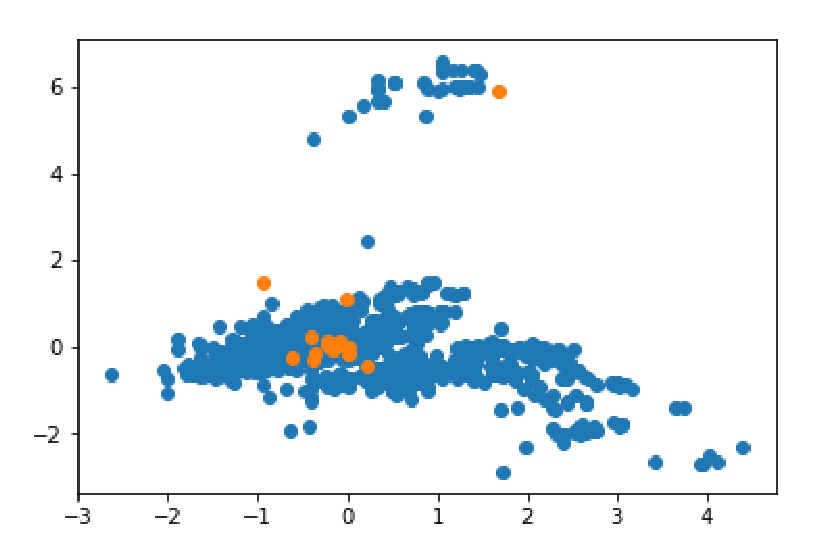
\includegraphics[scale=0.5]{figuras/pca.eps}
    \caption{Análise dos dados do \textit{LDA} utilizando \textit{PCA}}
\end{figure}

Os \textit{clusters} podem estar em mais de duas dimensões, porém analisando os nossos dados, mesmo em duas dimensões, conseguimos visualizar  apenas um \textit{cluster} separado e todo o resto junto, mostrando que a classificação claramente não está correta.

Tendo em vista o resultado acima, voltamos a utilizar o modelo \textit{naive Bayes} para realizar a classificação dos discursos e proposições.

\paragraph{Classificação dos Discursos e Proposições}

Como dito nos tópicos anteriores, serão utilizados os dados do \textit{thesaurus} da Câmara dos Deputados para o treinamento, a indexação dos discursos e proposições para e o classificador \textit{naive Bayes} para a análise.

Primeiramente, assim como na primeira parte do trabalho, é instanciado um objeto da classe \textit{NaiveBayesClassifier}, implementado pela biblioteca \textit{textblob}, passando como treinamento inicial o conjunto de termos já classificados do \textit{thesaurus}. Com o classificador treinado, passamos por cada discurso e em cada um deles obtemos a lista de termos usados em sua indexação. Cada termo é analisado individualmente e apenas aqueles que forem classificados com a probabilidade maior que 60\% são utilizados, o restante é descartado. Após classificar todos os termos de indexação de um discurso, calculamos a porcentagem de cada tema e atribuímos ao discurso. Por exemplo, suponha um discurso possui 13 termos na indexação e apenas 8 deles foram classificados com probabilidade maior que 60\%. Se 4 desses foram classificados como ``Segurança'', 3 como ``Direitos Humanos'' e 1 como ``Saúde'', então o discurso será classificado como sendo 50\% sobre segurança, 37,5\% direitos humanos e 12,5\% saúde. Além disso, definimos como tema principal do discurso aquele com maior porcentagem.

Vale enfatizar que as porcentagens mostradas pelo \textit{naive Bayes} são interpretadas de forma diferente que o \textit{LDA}. Enquanto no segundo trata-se de uma mistura de temas, no \textit{naive Bayes} correspondem à chance de um texto pertencer exclusivamente a cada tópico.

Para as proposições, os mesmos procedimentos são realizados, bem como a utilização do mesmo classificador já treinado.

\paragraph{Classificação dos Deputados}

Uma vez que todos os discursos e proposições estejam classificados, passamos por todos os deputados e em cada um deles obtemos uma lista de discursos e uma lista de proposições. Somamos todas as porcentagens, de todos os temas de discursos e proposições e dividimos pela soma da quantidade de discursos e proposições. Por exemplo, suponha que um parlamentar possui dois discursos e uma proposição classificada. Seu primeiro discurso é 100\% sobre ``Direitos Humanos'' e o segundo 70\% ``Saúde'' e 30\% ``Direitos Humanos''. A proposição foi classificada como 60\% ``Segurança'' e 40\% ``Educação''. Temos então que a classificação final do deputado seria: 43,3\% ``Direitos Humanos'', 23,3\% ``Saúde'', 20\% ``Segurança'' e 13,3\% ``Educação''. Assim como nos discursos e proposições, o tema com maior porcentagem é o tema principal de um deputado.

\paragraph{Classificação dos Estados}

Após a classificação dos deputados, passamos por todos os estados e em cada um obtemos a lista de parlamentares que o representam. Utilizando o mesmo procedimento da classificação dos deputados, somamos todas as porcentagens temáticas dos deputados e dividimos pela quantidade total de deputados.

\paragraph{Acurácia}

Após a mudança dos dados utilizados na análise, pudemos notar uma melhoria significativa no resultado da classificação. Utilizando como treinamento 11.151 termos, presentes no \textit{thesaurus}, e como teste 111 novos termos, obtidos da indexação dos próprios discursos e proposições, classificados manualmente pelo autor, obtivemos um índice de acerto de 59,46\%. Justificando, assim, a escolha de classificações apenas com probabilidade maior que 60\%, descrito nos itens anteriores.
